\subsection{Utility classes}

\begin{frame}[fragile]
  \frametitle{Core utility classes}
  \begin{itemize}
  \item Qt implements a core library of utility classes extensively used
    throughout the rest of the API.
  \begin{columns}
    \footnotesize
    \begin{column}{0.28\textwidth}
    \begin{itemize}
      \item \texttt{QString}
      \item \texttt{QByteArray}
      \item \texttt{QStringList}
      \item \texttt{QVector}
      \item \texttt{QList}
      \item \texttt{QLinkedList}
    \end{itemize}
    \end{column}
    \begin{column}{0.31\textheight}
    \begin{itemize}
      \item \texttt{QSet}
      \item \texttt{QMap}
      \item \texttt{QHash}
      \item \texttt{QVariant}
      \item \texttt{QDateTime}
      \item \texttt{QDir}
    \end{itemize}
    \end{column}
    \begin{column}{0.31\textheight}
    \begin{itemize}
      \item \texttt{QFileInfo}
      \item \texttt{QQFile}
      \item \texttt{QTextStream}
      \item \texttt{QDataStream}
      \item \texttt{QSerialPort}
      \item \ldots
    \end{itemize}
    \end{column}
  \end{columns}

  \item Project file \verb@QT += core@
  \end{itemize}
\end{frame}

\begin{frame}[fragile]
  \frametitle{\texttt{QString}\footnote
    {\url{http://doc.qt.io/qt-5.6/qstring.html}}}
  \begin{itemize}
    \item Class for storing, transferring and manipulating text in the form of
      zero-terminated character strings.
    \item Internally stores the strings in 16-bit wide \texttt{QChar}s using
      the UTF-16\footnote{\url{https://en.wikipedia.org/wiki/UTF-16}} encoding.
    \begin{itemize}
      \item Note that glyphs with Unicode code-points above $2^{16}$ are
        represented by multi-\texttt{QChar} sequences!
    \end{itemize}
    \item May use copy-on-write to reduce memory usage and to avoid the needless
      copying of data.
    \item Header \verb@#include<QString>@
  \end{itemize}
\end{frame}

\begin{frame}[fragile]
  \frametitle{\texttt{QString} -- initialization}
  \begin{itemize}
    \item Can be initialized from UTF-8\footnote
     {\url{https://en.wikipedia.org/wiki/UTF-8}}-encoded c-string literals or
     \texttt{char} arrays.
    \begin{itemize}
      \item
      \begin{verbatim}
	QString str = "hello!";
      \end{verbatim}
      \item internally calls \verb@QString::fromUtf8@.
    \end{itemize}
    \item \texttt{QStringLiteral} -- a potentially more efficient variant of
      the above. Can do the conversion to the internal implementation at
      compile-time.
    \begin{itemize}
      \item
      \begin{verbatim}
	QString str = QStringLiteral("hello!");
      \end{verbatim}
      \item only if the compiler supports it.
    \end{itemize}
    \item Also can be initialized from arrays of \texttt{QChar}s.
    \begin{itemize}
      \item
      \begin{verbatim}
	const QChar strdata[N] = {0x0055, ...};
	QString str(strdata, N);
      \end{verbatim}
    \end{itemize}
  \end{itemize}
\end{frame}

\begin{frame}[fragile]
  \frametitle{\texttt{QString} -- null vs. empty}
  \small
  \begin{itemize}
    \item Qt distinguishes between {\em null} and {\em empty} strings.
    \begin{itemize}
      \item {\em null}-string -- default-initialized or initialized from a
      \texttt{nullptr}.
      \item {\em empty}-string -- initialized from a string containing only
      the terminating zero character.
      \item {\em nonempty}-string -- any other string.
    \end{itemize}
    \item
    \begin{lstlisting}
	QString null;
	QString empty("");
	QString nonempty("abc");

	assert(null.isNull()     == true);
	assert(empty.isNull()    == false);
	assert(nonempty.isNull() == false);

	assert(null.isEmpty()    == true);
	assert(empty.isEmpty()   == true);
	assert(nonempty.isEmpty()== false);
      \end{lstlisting}
  \end{itemize}
\end{frame}

\begin{frame}[fragile]
  \frametitle{\texttt{QByteArray}\footnote
    {\url{http://doc.qt.io/qt-5.6/qbytearray.html}}}
  \begin{itemize}
    \item Class for storing, transferring and manipulating raw byte sequences,
      including text encoded in UTF-8 and other 8-bit character encodings.
    \item Can be more efficient to store texts in some character sets\footnote
    {like basic Latin} if memory resources are constrained.
    \begin{itemize}
      \item Otherwise \texttt{QString} is the preferred and recommended way to
      store text.
    \end{itemize}
    \item The data can embed zero characters.
    \item If initialized from a char array, terminating zero is preserved.

    \item Header \verb@#include<QByteArray>@
  \end{itemize}
\end{frame}

\begin{frame}[fragile]
  \frametitle{\texttt{QByteArray} -- initialization}
  \begin{itemize}
    \item Can be initialized from
    \begin{itemize}
      \item a c-string literal:
      \begin{verbatim}
	QByteArray ba("some text");
      \end{verbatim}
      \item a raw memory block:
      \begin{verbatim}
	const char raw[N] = {0x00, ...};
	QByteArray ba = QByteArray::fromRawData(raw,N);
      \end{verbatim}
      \item a \verb@std::string@:
      \begin{verbatim}
	std::string str(...);
	QByteArray ba = QByteArray::fromStdString(str);
      \end{verbatim}
      \item \ldots
    \end{itemize}
  \end{itemize}
\end{frame}

\begin{frame}[fragile]
  \frametitle{\texttt{QString}, \texttt{QByteArray} -- manipulation}
  \footnotesize
  \begin{itemize}
    \item \verb@data@ -- returns a pointer to the stored data.
    \item \verb@size@, \verb@length@ -- returns the size (in bytes) of the
    stored data.
    \item \verb@resize@ -- resizes the internally allocated memory block.
    \item \verb@capacity@ -- returns the capacity of the allocated memory block.
    \item \verb@clear@
    \item \verb@begin@, \verb@end@ -- return iterators to the first and past
    the last byte.
    \item \verb@at@ -- returns the character at the specified index.
    \item \verb@operator[]@ -- returns a reference to the character at the
    specified index.
    \item \verb@isNull@, \verb@isEmpty@
    \item \verb@prepend@, \verb@append@, \verb@insert@, \verb@replace@
    \item \verb@startsWith@, \verb@endsWith@, \verb@contains@, \verb@indexOf@
    \item \verb@left@, \verb@right@, \verb@mid@, \verb@chop@, \verb@truncate@
    \item \ldots
  \end{itemize}
\end{frame}

\begin{frame}[fragile]
  \frametitle{\texttt{QString}, \texttt{QByteArray} -- conversions}
  \small
  \begin{itemize}
    \item \verb@QString::utf16@ -- pointer to the internal representation.
    \item \verb@QString::setUtf16@ -- replace the contents with a new UTF-16 string.
    \item \verb@QString::toUtf8@ -- returns a UTF-8 encoded \verb@QByteArray@.
    \item \verb@QString::fromUtf8@
    \item \verb@QString::fromLatin1@, \verb@QString::toLatin1@
    \item \verb@QString::fromUcs4@, \verb@QString::toUcs4@
    \item \verb@QString::fromLocal8Bit@, \verb@QString::toLocal8Bit@
    \item \verb@QString::fromStdString@, \verb@fromStdU16String@,
    \verb@fromStdU32String@, \verb@fromStdWString@
    \item \verb@QString::toStdString@, \verb@toStdU16String@,
    \verb@toStdU32String@, \verb@toStdWString@
    \item \ldots
  \end{itemize}
\end{frame}

\begin{frame}[fragile]
  \frametitle{\texttt{QString} -- formatting}
  \begin{itemize}
    \item String containing several instances of the placeholder \verb@%N@,
    where \verb@N@ is a natural number, starting from one
    \item chain of calls to \verb@QString::arg@ specifying the values
    to replace the placeholders.
    \begin{lstlisting}
	QString format("Iteration %1 of %2 - %3 %");

	for(int i=0, n=10; i<=n; ++i)
	{
	    qDebug() << format
	        .arg(i, 2)
	        .arg(n, 2)
	        .arg(100*float(i)/n, 3);
	}
    \end{lstlisting}
  \end{itemize}
\end{frame}

\begin{frame}[fragile]
  \frametitle{\texttt{QStringList}\footnote
    {\url{http://doc.qt.io/qt-5.6/qstringlist.html}}}
  \begin{itemize}
    \item \texttt{QStringList} implements an efficient, ordered, random-access
    sequence of \texttt{QString}s.
    \item Inherits from \verb@QList<QString>@\footnote{More on that later}.
    \begin{itemize}
      \item provides random access,
      \item provides several other methods of element iteration.
      \item efficient implementation,
      \item may use copy-on-write to prevent unnecessary copying.
    \end{itemize}
    \item Adds functionality specific to sequences of strings:
    \begin{itemize}
      \item syntax sugar for initialization,
      \item split and join\footnote{Similar to Python's},
      \item \ldots
    \end{itemize}
    \item Header \verb@#include<QStringList>@
  \end{itemize}
\end{frame}

\begin{frame}[fragile]
  \frametitle{\texttt{QStringList} -- iteration}
  \small
  \begin{itemize}
    \item Indexing:
     \begin{lstlisting}
	QStringList items(...); 
	for(int i = 0; i < items.size(); ++i)
	{
	    qDebug() << items.at(i);
	}
     \end{lstlisting}
    \item Java-style iteration:
     \begin{lstlisting}
	QStringList items(...); 
	QStringListIterator iter(items);
	while(iter.hasNext())
	{
	    qDebug() << iter.next();
	}
     \end{lstlisting}
  \end{itemize}
\end{frame}

\begin{frame}[fragile]
  \frametitle{\texttt{QStringList} -- iteration (cont.)}
  \small
  \begin{itemize}
    \item STL-style iterator
     \begin{lstlisting}
	QStringList items(...); 
	QStringList::const_iterator iter = items.begin();
	while(iter != items.end())
	{
	    qDebug() << *(iter++);
	}
     \end{lstlisting}
  \end{itemize}
  \begin{columns}
    \begin{column}{0.55\textwidth}
    \begin{itemize}
    \item Qt's \texttt{foreach}:
     \begin{lstlisting}[basicstyle=\scriptsize\ttfamily]
	QStringList items(...); 
	foreach(QString item, items)
	{
	    qDebug() << item;
	}
     \end{lstlisting}
    \end{itemize}
    \end{column}
    \begin{column}{0.47\textwidth}
    \begin{itemize}
    \item C++11 range-based \texttt{for}:
     \begin{lstlisting}[basicstyle=\scriptsize\ttfamily]
	QStringList items(...); 
	for(QString item: items)
	{
	    qDebug() << item;
	}
     \end{lstlisting}
    \end{itemize}
    \end{column}
  \end{columns}
\end{frame}

\begin{frame}[fragile]
  \frametitle{\texttt{QString}, \texttt{QStringList} -- split}
    \texttt{QString::split} -- splits a \texttt{QString} into a \texttt{QStringList}
     of substrings on every occurence of a separator character or substring.

    \vfill

    \begin{columns}
    \begin{column}{0.75\textwidth}
       \begin{lstlisting}
	QString itemstr("A,B,C,,D,E,F");
	QStringList items = itemstr.split(',');

	foreach(QString item, items)
	{
	    qDebug() << item;
	}
       \end{lstlisting}
    \end{column}
    \begin{column}{0.25\textwidth}
       \small
       Prints the following output:
       \begin{verbatim}
	"A"
	"B"
	"C"
	""
	"D"
	"E"
	"F"
       \end{verbatim}
    \end{column}
  \end{columns}
\end{frame}

\begin{frame}[fragile]
  \frametitle{\texttt{QString}, \texttt{QStringList} -- join}
    \texttt{QStringList::join} -- joins the individual strings in a
    \texttt{QStringList} into a single string with the substrings delimited
    by a separator character or string.

    \begin{lstlisting}
	QStringList items;
	items << "A" << "B" << "C" << "" << "D" << "E" << "F";

	qDebug() << items.join(", ");
	qDebug() << items.join("/");
    \end{lstlisting}
     \small
     Prints the following output:
    \begin{verbatim}
	"A, B, C, , D, E, F"
	"A/B/C//D/E/F"
    \end{verbatim}
\end{frame}

\begin{frame}
  \frametitle{Generic containers}
  \begin{itemize}
    \item General-purpose, templated containers storing homogeneous elements
    of specified type.
    \item Most commonly used:
    \begin{itemize}
      \item \texttt{QVector}, \texttt{QList}, \texttt{QLinkedList}
      \item \texttt{QSet}, \texttt{QMap}, \texttt{QHash}
      \item \texttt{QQueue}, \texttt{QStack}
    \end{itemize}
    \item but also:
    \begin{itemize}
      \item \texttt{QVarLengthArray}
      \item \texttt{QMultiMap}, \texttt{QMultiHash}
    \end{itemize}
    \item inspired by the STL containers,
    \item some groups of containers like \texttt{QVector} and \texttt{QList}
    implement similar interfaces,
    \item but have different performance and iterator invalidation characteristics.
  \end{itemize}
\end{frame}

\begin{frame}[fragile]
  \frametitle{\texttt{QVector}
    \footnote{\url{http://doc.qt.io/qt-5.6/qvector.html}}}
  \begin{itemize}
    \item \texttt{QVector<T>} is a generic random-access sequence of elements of
    type \texttt{T} with contiguous storage of its elements.
    \item Usually gives better performance on modern CPUs than \texttt{QList}.
    \item Constant-time random access to elements.
    \item Linear-time element insertion and removal.
    \item Constant-time append.
    \item Insertion and removal invalidates iterators.
    \item The recommended generic container since Qt version 5.6.
    \item Will probably gradually replace \texttt{QList} in the future.
    \item Header \verb@#include<QVector>@
    \item STL equivalent: \verb@std::vector@
  \end{itemize}
\end{frame}

\begin{frame}[fragile]
  \frametitle{\texttt{QList}\footnote
    {\url{http://doc.qt.io/qt-5.6/qlist.html}}}
  \begin{itemize}
    \item \texttt{QList<T>} is a generic random-access sequence of elements of
    type \texttt{T} which does not guarantee contiguous storage of its elements.
    \item \say{Fast} indexed element lookup.
    \item \say{Fast} element insertion and removal.
    \item May or may not allocate storage on the heap.
    \item Iterator invalidation and performance depends on how the storage
    is allocated.
    \item Qt recommends to use \texttt{QVector} or \texttt{QLinkedList}
    where possible in new code.
    \item However, \texttt{QList} is used frequently in the API and legacy
    code-base.
    \item Header \verb@#include<QList>@
  \end{itemize}
\end{frame}

\begin{frame}[fragile]
  \frametitle{\texttt{QLinkedList}\footnote
    {\url{http://doc.qt.io/qt-5.6/qlinkedlist.html}}}
  \begin{itemize}
    \item \texttt{QList<T>} is a generic forward sequence of elements of
    type \texttt{T} where the storage space for each element is typically
    allocated separately.
    \item Implemented as a linked list.
    \item Linear-time indexed element lookup.
    \item Constant-time element insertion and removal.
    \item May lead to memory fragmentation.
    \item Header \verb@#include<QLinkedList>@
    \item STL equivalent: \verb@std::list@
  \end{itemize}
\end{frame}

\begin{frame}[fragile]
  \frametitle{\texttt{QSet}\footnote
    {\url{http://doc.qt.io/qt-5.6/qset.html}}}
  \begin{itemize}
    \item \texttt{QSet<T>}
    \item Implements a hash table-based set.
    \item Very fast element lookup, insertion and removal -- typically
      constant-time.
    \item The element type must provide \verb@operator ==@.
    \item The element type must provide a global hash function \verb@qHash@.
    \item Iterated elements {\em are not} ordered.
    \item Header \verb@#include<QSet>@
    \item STL equivalent: \verb@std::unordered_set@
  \end{itemize}
\end{frame}

\begin{frame}[fragile]
  \frametitle{\texttt{QMap}\footnote
    {\url{http://doc.qt.io/qt-5.6/qmap.html}}}
  \begin{itemize}
    \item \texttt{QMap<Key, T>}
    \item Implements a hash red-black tree-based dictionary.
    \item Logarithmic-time element lookup, insertion and removal.
    \item The \verb@Key@ type must provide \verb@operator <@.
    \item Iterated elements are ordered according to the result of the
    \verb@operator <@ on the values of \verb@Key@.
    \item Header \verb@#include<QMap>@
    \item STL equivalent: \verb@std::map@
  \end{itemize}
\end{frame}

\begin{frame}[fragile]
  \frametitle{\texttt{QHash}\footnote
    {\url{http://doc.qt.io/qt-5.6/qhash.html}}}
  \begin{itemize}
    \item \texttt{QHash<Key, T>}
    \item Implements a hash table-based dictionary.
    \item Element lookup, insertion and removal usually faster than \texttt{QMap}
    and typically constant-time.
    \item The \verb@Key@ type must provide \verb@operator ==@.
    \item The \verb@Key@ type must provide a hash function \verb@qHash@.
    \item Iterated elements are not ordered.
    \item Header \verb@#include<QHash>@
    \item STL equivalent: \verb@std::unordered_map@
  \end{itemize}
\end{frame}

\begin{frame}[fragile]
  \frametitle{\texttt{QVariant}
    \footnote{\url{http://doc.qt.io/qt-5.6/qvariant.html}}}
  \begin{itemize}
    \item Similar to a \say{smart} \verb@union@ for most common Qt types.
    \item Provides single-parameter constructor and assignment operators
      for many comonly used C++ native or Qt types.
    \item Allows to store and pass around values of heterogeneous types by
      using a single type.
    \item Allows to retrieve the value in the original type.
    \item If possible allows to convert the value into a different type.
    \item Allows to write the value to an output stream.
    \item Header \verb@#include<QVariant>@
  \end{itemize}
\end{frame}

\begin{frame}[fragile]
  \frametitle{\texttt{QVariant} -- basic usage}
  \small
  \begin{columns}
    \begin{column}{0.47\textwidth}
    \begin{lstlisting}
	QVariant v;
	qDebug() << v.isNull();

	v = 123;
	qDebug() << v.isNull();
	qDebug() << v.typeName();
	qDebug() << v;
	qDebug() << v.toInt();
	qDebug() << v.toBool();

	v = 0;
	qDebug() << v.toBool();

	v = QByteArray("blable");
	qDebug() << v;
    \end{lstlisting}
    \end{column}
    \begin{column}{0.53\textwidth}
    \begin{lstlisting}
	QVector<QVariant> vv;

	vv.push_back(12);
	vv.push_back(34.56);
	vv.push_back("789");
	vv.push_back(false);

	foreach(QVariant x, vv)
	{
	    qDebug() << x;
	}
    \end{lstlisting}
    \end{column}
  \end{columns}
\end{frame}

\begin{frame}[fragile]
  \frametitle{\texttt{QDate}
    \footnote{\url{http://doc.qt.io/qt-5.6/qdate.html}}}
  \small
  \begin{itemize}
    \item Stores and manipulates dates (year, month, day) in the Gregorian
      calendar.
    \item Construction:
    \begin{itemize}
      \footnotesize
      \item \verb@QDate date(2016, 5, 16);@
      \item \verb@QDate::currentDate();@
      \item \verb@QDate::fromString("20000110", "yyyyMMdd");@
    \end{itemize}
    \item Operations
    \begin{columns}
      \scriptsize
      \begin{column}{0.4\textwidth}
      \begin{itemize}
        \item \verb@year@, \verb@month@, \verb@day@
        \item \verb@addYears@, \verb@addMonths@, \verb@addDays@
        \item \verb@weekNumber@, \verb@dayOfWeek@, \verb@dayOfYear@
        \item \verb@daysInMonth@, \verb@daysInYear@
      \end{itemize}
      \end{column}
      \begin{column}{0.4\textwidth}
      \begin{itemize}
        \item \verb@isLeapYear@
        \item \verb@isValid@, \verb@isNull@
        \item \verb@shortDayName@, \verb@longDayName@
        \item \verb@shortMonthName@, \verb@longMonthName@
      \end{itemize}
      \end{column}
    \end{columns}
    \item Header \verb@#include<QDate>@
  \end{itemize}
\end{frame}

\begin{frame}
  \frametitle{Date format strings}
  \scriptsize
  \begin{center}
  \rowcolors{2}{green!80!yellow!50}{green!70!yellow!40}
  \begin{tabular}{|p{0.13\textwidth}|p{0.77\textwidth}|}
    \hline
    \textbf{String} & \textbf{Output} \\
    \hline
    d & the day as number without a leading zero (1 to 31) \\
    \hline
    dd & the day as number with a leading zero (01 to 31) \\
    \hline
    ddd & the abbreviated localized day name (e.g. 'Mon' to 'Sun'). \\
    \hline
    dddd & the long localized day name (e.g. 'Monday' to 'Sunday'). \\
    \hline
    M & the month as number without a leading zero (1-12) \\
    \hline
    MM & the month as number with a leading zero (01-12) \\
    \hline
    MMM & the abbreviated localized month name (e.g. 'Jan' to 'Dec'). \\
    \hline
    MMMM & the long localized month name (e.g. 'January' to 'December'). \\
    \hline
    yy & the year as two digit number (00-99) \\
    \hline
    yyyy & the year as four digit number \\
    \hline
  \end{tabular}
  \end{center}
\end{frame}

\begin{frame}[fragile]
  \frametitle{\texttt{QTime}
    \footnote{\url{http://doc.qt.io/qt-5.6/qtime.html}}}
  \begin{itemize}
    \item Stores and manipulates day-times (hours, minutes, seconds and
      milliseconds) since the midnight.
    \item No notion of timezone and DST
    \item Construction:
    \begin{itemize}
      \footnotesize
      \item \verb@QTime time(10, 15, 30); // 10:15:30.000@
      \item \verb@QTime::currentTime();@
      \item \verb@QTime::fromString("10:00:00", "hh:mm:ss");@
    \end{itemize}
    \item Operations
    \begin{columns}
      \scriptsize
      \begin{column}{0.4\textwidth}
      \begin{itemize}
        \item \verb@hour@, \verb@minute@, \verb@second@, \verb@msec@
        \item \verb@addHours@, \verb@addMinutes@, \verb@addSecs@, \verb@addMSecs@
      \end{itemize}
      \end{column}
      \begin{column}{0.4\textwidth}
      \begin{itemize}
        \item \verb@isValid@, \verb@isNull@
        \item \verb@start@, \verb@restart@, \verb@elapsed@
        \item \verb@toString@
        \item \ldots
      \end{itemize}
      \end{column}
    \end{columns}
    \item Header \verb@#include<QTime>@
  \end{itemize}
\end{frame}

\begin{frame}
  \frametitle{Time format strings}
  \scriptsize
  \begin{center}
  \rowcolors{2}{green!80!yellow!50}{green!70!yellow!40}
  \begin{tabular}{|p{0.13\textwidth}|p{0.77\textwidth}|}
    \hline
    \textbf{String} & \textbf{Output} \\
    \hline
    h & the hour without a leading zero (0 to 23 or 1 to 12 if AM/PM display) \\
    \hline
    hh & the hour with a leading zero (00 to 23 or 01 to 12 if AM/PM display) \\
    \hline
    H & the hour without a leading zero (0 to 23, even with AM/PM display) \\
    \hline
    HH & the hour with a leading zero (00 to 23, even with AM/PM display) \\
    \hline
    m & the minute without a leading zero (0 to 59) \\
    \hline
    mm & the minute with a leading zero (00 to 59) \\
    \hline
    s & the second without a leading zero (0 to 59) \\
    \hline
    ss & the second with a leading zero (00 to 59) \\
    \hline
    z & the milliseconds without leading zeroes (0 to 999) \\
    \hline
    zzz & the milliseconds with leading zeroes (000 to 999) \\
    \hline
    AP or A & interpret as an AM/PM time. AP must be either "AM" or "PM". \\
    \hline
    ap or a & Interpret as an AM/PM time. ap must be either "am" or "pm". \\
    \hline
  \end{tabular}
  \end{center}
\end{frame}

\begin{frame}[fragile]
  \frametitle{\texttt{QDateTime}
    \footnote{\url{http://doc.qt.io/qt-5.6/qdatetime.html}}}
  \begin{itemize}
    \item Stores and manipulates dates and times.
    \item Knows about timezones and DST
    \item Construction:
    \begin{itemize}
      \footnotesize
      \item \verb@QDateTime dt(QDate(...), QTime(...));@
      \item \verb@QDateTime::currentDateTime();@
      \item \verb@QDateTime::currentDateTimeUtc();@
      \item \verb@QDateTime::fromString("2015-05-16 10:00:00", format);@
    \end{itemize}
    \item Operations
    \begin{columns}
      \scriptsize
      \begin{column}{0.4\textwidth}
      \begin{itemize}
        \item same as \texttt{QDate} and \texttt{QTime}
        \item \verb@setDate@, \verb@setTime@, \verb@setTimeZone@
        \item \verb@date@, \verb@time@, \verb@timeSpec@, \verb@timeZone@
      \end{itemize}
      \end{column}
      \begin{column}{0.4\textwidth}
      \begin{itemize}
        \item \verb@isDaylightTime@
        \item \verb@toUtc@, \verb@toLocalTime@, \verb@toTimeZone@
        \item \verb@toString@
      \end{itemize}
      \end{column}
    \end{columns}
    \item Header \verb@#include<QDateTime>@
  \end{itemize}
\end{frame}

\begin{frame}[fragile]
  \frametitle{\texttt{QTimeZone}
    \footnote{\url{http://doc.qt.io/qt-5.6/qtimezone.html}}}
  \begin{itemize}
    \item Represents global time zones\footnote
     {\url{http://www.iana.org/time-zones}}
    \item Allows conversions between times in UTC and a particular time zone
    \item Construction:
    \begin{itemize}
      \scriptsize
      \item \verb@QTimeZone tz(+3600);@
      \item \verb@QTimeZone tz(-7*3600);@
      \item \verb@QTimeZone tz("Europe/Berlin");@
      \item \verb@QTimeZone::utc();@
      \item \verb@QTimeZone::systemTimeZone();@
    \end{itemize}
    \item Operations
    \begin{columns}
      \scriptsize
      \begin{column}{0.4\textwidth}
      \begin{itemize}
        \item \verb@id@, \verb@displayName@, \verb@abbreviation@, \verb@comment@
        \item \verb@country@
        \item \verb@availableTimeZoneIds@
      \end{itemize}
      \end{column}
      \begin{column}{0.4\textwidth}
      \begin{itemize}
        \item \verb@offsetFromUtf@, \verb@standardTimeOffset@
        \item \verb@hasDaylightTime@, \verb@hasTransitions@
        \item \ldots
      \end{itemize}
      \end{column}
    \end{columns}
    \item Header \verb@#include<QTimeZone>@
  \end{itemize}
\end{frame}

\begin{frame}[fragile]
  \frametitle{\texttt{QDir}
    \footnote{\url{http://doc.qt.io/qt-5.6/qdir.html}}}
  \begin{itemize}
    \item \texttt{QDir} -- provides file system directory tree traversal and
     manipulation functionality.
    \item Can also be used to access the Qt's resource system.
    \item Allows access to entities managed by a file system by the means of
      {\em paths}:
      \begin{itemize}
        \item Structured strings
        \item Use the forward-slash \say{\texttt{/}} as an universal,
        platform-independent separator.
        \item However paths are still partially platform-dependent.
        \item Absolute
        \item Relative
      \end{itemize}
    \item Header \verb@#include<QDir>@
  \end{itemize}
\end{frame}

\begin{frame}[fragile]
  \frametitle{\texttt{QDir} -- construction}
  \small
  \begin{itemize}
    \item From a path-string
    \begin{itemize}
    \item Absolute:
    \begin{verbatim}
	QDir unix_dir("/usr/local/include");
	QDir win_dir1("C:/Windows/system32/drivers");
	QDir win_dir2("C:\\Windows\\system32\\drivers");
    \end{verbatim}
    \item Relative:
    \begin{verbatim}
	QDir rel_dir1("file.txt");
	QDir rel_dir2("./file.txt");
	QDir rel_dir3("../file.txt");
	QDir rel_dir4("subdir/file.txt");
	QDir rel_dir5("../dir/file.txt");
    \end{verbatim}
    \end{itemize}
    \item The stored path as string:
    \begin{verbatim}
	QDir dir(...);
	QString str = dir.path();
    \end{verbatim}
  \end{itemize}
\end{frame}

\begin{frame}[fragile]
  \frametitle{\texttt{QDir} -- basic operations}
  \footnotesize
  \begin{columns}
    \begin{column}{0.45\textwidth}
    \begin{itemize}
      \item Testing if absolute or relative
      \begin{itemize}
      \item \verb@QDir::isAbsolute@
      \item \verb@QDir::isRelative@
      \end{itemize}
      \item Getting path components
      \begin{itemize}
        \item \verb@dirName@
      \end{itemize}
      \item \texttt{QDir}s of special directories
      \begin{itemize}
        \item \verb@current@ -- current working directory
        \item \verb@home@ -- current user's home directory
        \item \verb@root@ -- file system root directory
        \item \verb@temp@ -- temporary directory
      \end{itemize}
    \end{itemize}
    \end{column}
    \begin{column}{0.55\textwidth}
    \begin{itemize}
      \item Path \texttt{QStrings} to special directories
      \begin{itemize}
        \item \verb@currentPath@
        \item \verb@homePath@
        \item \verb@rootPath@
        \item \verb@tempPath@
      \end{itemize}
      \item Resolving paths
      \begin{itemize}
        \item \verb@absolutePath@ -- in relation to current directory.
        \item \verb@cleanPath@ -- removes redundant components like  \texttt{.},
          \texttt{..} and \texttt{/}, but preserves symbolic links.
        \item \verb@canonicalPath@ -- returns an absolute path, but also removes
          redundant components and resolves symbolic links.
      \end{itemize}
    \end{itemize}
    \end{column}
  \end{columns}
\end{frame}

\begin{frame}[fragile]
  \frametitle{\texttt{QDir} -- FS navigation, inspection and manipulation}
  \footnotesize
  \begin{columns}
    \begin{column}{0.55\textwidth}
    \begin{itemize}
      \item Navigation
      \begin{itemize}
        \item \verb@QDir::cd@ -- tries to change the {\em cwd} to the specified
        directory
        \item \verb@QDir::cdUp@ -- tries to change the {\em cwd} to the parent
        directory
      \end{itemize}
      \item Testing directory properties
      \begin{itemize}
        \item \verb@exists@ -- directory exists
        \item \verb@isRoot@ -- directory is root
        \item \verb@isReadable@ -- directory is readable
      \end{itemize}
      \item Platform-specific
      \begin{itemize}
        \item \verb@separator@ -- native path separator
        \item \verb@listSeparator@ -- native path list separator
      \end{itemize}
    \end{itemize}
    \end{column}
    \begin{column}{0.45\textwidth}
    \begin{itemize}
      \item Directory manipulation
      \begin{itemize}
        \item \verb@mkdir@ -- must not exist
        \item \verb@rmdir@ -- must be empty
        \item \verb@mkpath@ -- creates parent directories if unnecessary
        \item \verb@rmpath@ -- recursively removes if all subdirs are empty
        \item \verb@remove@ -- remove file
        \item \verb@removeRecursively@ -- remove whole subtree
        \item \verb@rename@
      \end{itemize}
    \end{itemize}
    \end{column}
  \end{columns}
\end{frame}

\begin{frame}[fragile]
  \frametitle{\texttt{QDir} -- file system entry enumeration}
  \begin{itemize}
    \item Enumeration functions
    \begin{itemize}
      \item \verb@drives@ -- list of all root directories on the system
      \item \verb@count@ -- total number of entries in the directory
      \item \verb@entryList@ -- a \texttt{QStringList} of names of entries
      \item \verb@entryInfoList@ -- a \texttt{QFileInfoList} of entries
    \end{itemize}
    of the directory
    \item Filter configuration functions
    \begin{itemize}
      \item \verb@setFilter@
      \item \verb@setNameFilters@
      \item \verb@setSorting@
    \end{itemize}
  \end{itemize}
\end{frame}

\begin{frame}[fragile]
  \frametitle{\texttt{QFileInfo}
    \footnote{\url{http://doc.qt.io/qt-5.6/qfileinfo.html}} and
    \texttt{QFileInfoList}}
  \begin{itemize}
    \item \texttt{QFileInfo} -- provides file system entry status checking
      functionality.
    \begin{itemize}
      \item file system path
      \item path components
      \item whether it exists
      \item entry kind (directory, file, symbolic link, device, etc.)
      \item ownership and permissions
      \item access and modification times
    \end{itemize}
    \item \texttt{QFileInfoList} -- list of file info instances
    \begin{itemize}
      \item \verb@typedef QList<QFileInfo> QFileInfoList@
    \end{itemize}
    \item Header \verb@#include<QFileInfo>@
  \end{itemize}
\end{frame}

\begin{frame}[fragile]
  \frametitle{\texttt{QFile}
    \footnote{\url{http://doc.qt.io/qt-5.6/qfile.html}}}
  \begin{itemize}
    \item \texttt{QFile} -- provides file reading and writing functionality.
    \item May be used by itself or more conveniently with \texttt{QTextStream}
      or \texttt{QDataStream}.
    \item Basic \verb@seek@, \verb@read@ and \verb@write@ operations inherited
      from \texttt{QFileDevice}.
    \item Also supports basic file system operations like \verb@rename@,
      \verb@remove@, \verb@link@, \verb@exists@, symbolic link resolution,
      permission setup, etc.
  
    \item Header \verb@#include<QFile>@
  \end{itemize}
\end{frame}

\begin{frame}[fragile]
  \frametitle{\texttt{QFile} -- reading text file directly}

  \begin{lstlisting}[basicstyle=\small\ttfamily]
	QFile file("file.txt");

	if(!file.open(QFile::ReadOnly | QFile::Text))
	{
	    reportFileError(...);
	}

	while(!file.atEnd())
	{
	    QByteArray line = file.readLine();
	    processLine(line);
	}
  \end{lstlisting}
\end{frame}

\begin{frame}[fragile]
  \frametitle{\texttt{QTextStream}
    \footnote{\url{http://doc.qt.io/qt-5.6/qtextstream.html}}}
  \begin{itemize}
    \item \texttt{QTextStream} -- provides a convenient interface for reading
    and writing text data streams.
    \item Implements stream insertion and extraction operators \verb@>>@ and \verb@<<@.
    \item Implements stream manipulators:
    \begin{itemize}
      \item \verb@endl@, \verb@flush@
      \item \verb@dec@, \verb@bin@, \verb@hex@, \verb@oct@
      \item \verb@scientific@
      \item \verb@left@, \verb@right@
      \item \verb@qSetFieldWidth@, \verb@qSetPadChar@
      \item \ldots
    \end{itemize}
    \item Header \verb@#include<QTextStream>@
  \end{itemize}
\end{frame}

\begin{frame}[fragile]
  \frametitle{\texttt{QFile} -- writing text file with \texttt{QTextStream}}
  \begin{lstlisting}

	QFile file(QDir::temp()+"/test.txt");

	if(file.exists())
	{
	    file.remove();
	}

	if(file.open(QFile::WriteOnly | QFile::Truncate))
	{
	    QTextStream fout(&file);
	    fout << "Blah\n";
	    fout << qSetFieldWidth(10) << left << 3.14 << 1234;
	}
	file.close();
  \end{lstlisting}
\end{frame}

\begin{frame}[fragile]
  \frametitle{\texttt{QDataStream}
    \footnote{\url{http://doc.qt.io/qt-5.6/qdatastream.html}}}
  \begin{itemize}
    \item \texttt{QDataStream} -- provides a convenient interface for reading
    and writing cross-platform raw data streams.
    \item Data is encoded into streams which are host platform- and byte
      order-independent.
    \item Implements stream insertion and extraction operators \verb@>>@ and \verb@<<@
      for basic C++ types.
    \item Structured types can be serialized by (recursively) breaking them up
      into smaller units up the the basic types.
    \item Versioning allows the stream format to evolve while maintaining
     version information.
    \item Header \verb@#include<QDataStream>@
  \end{itemize}
\end{frame}

\begin{frame}[fragile]
  \frametitle{\texttt{QIODevice}
    \footnote{\url{http://doc.qt.io/qt-5.6/qiodevice.html}}}
  \small
  \begin{columns}
    \begin{column}{0.68\textwidth}
    \begin{itemize}
    \item \texttt{QIODevice} -- is a base class for various input/output devices,
      capable of reading and writing blocks of data.
    \begin{itemize}
      \item{QFileDevice}
      \item{QSerialPort}
      \item{QTcpSocket}
      \item{QLocalSocket}
      \item{QAbstractSocket}
      \item{QBluetoothSocket}
      \item \ldots
    \end{itemize}
    \item Implements basic operations read, write, seek and wait I/O operations.
    \item Header \verb@#include<QFile>@
    \end{itemize}
    \end{column}
    \begin{column}{0.32\textwidth}
    \begin{figure}[!t]
    \centering
    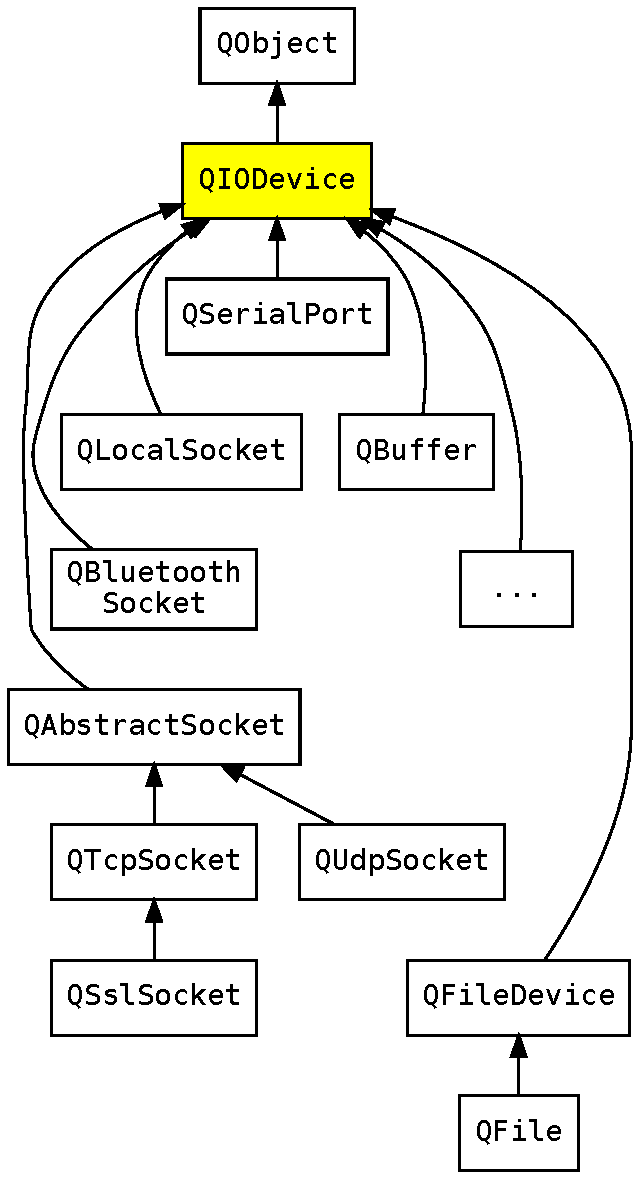
\includegraphics[width=\textwidth]{images/qiodevice.pdf}
    \end{figure}
    \end{column}
  \end{columns}
\end{frame}

\begin{frame}[fragile]
  \frametitle{\texttt{QSerialPort}
    \footnote{\url{http://doc.qt.io/qt-5.6/qserialport.html}}}
  \begin{itemize}
    \item \texttt{QSerialPort} -- specialization of \texttt{QIODevice} for
      the communication through serial interfaces.
    \begin{itemize}
      \item \verb@baudRate@
      \item \verb@parity@
      \item \verb@dataBits@
      \item \verb@stopBits@
      \item \verb@flowControl@
      \item \verb@pinoutSignals@
      \item \verb@requestToSend@
      \item \verb@clear@
      \item \ldots
    \end{itemize}
    \item Always opened with exclusive access.
    \item Header \verb@#include<QSerialPort>@
  \end{itemize}
\end{frame}

\begin{frame}[fragile]
  \frametitle{\texttt{QCoreApplication}
    \footnote{\url{http://doc.qt.io/qt-5.6/qcoreapplication.html}}}
    \small
    \begin{itemize}
      \item Provides an event loop for applications without a graphics UI.
      \begin{itemize}
        \item system timer events
        \item network events
        \item \ldots
        \item \texttt{exec}, \texttt{quit}
      \end{itemize}
      \item A non-GUI application should use at most one instance of this class.
      \item Is a \texttt{QObject} with signals\footnote{More on that later}.
      \item Handles application initialization and cleanup.
      \item Provides basic access to command-line arguments and executable path.
      \item Manages application localization settings.
      \item Interacts with \texttt{QSettings} and the management of system-wide
        and application-wide settings.
    \end{itemize}
\end{frame}

\begin{frame}[fragile]
  \frametitle{\texttt{QSettings}
    \footnote{\url{http://doc.qt.io/qt-5.6/qsettings.html}}}
  \small
  \begin{itemize}
    \item \texttt{QSettings} -- implements a platform-independent abstraction
      for persistent application settings store.
      \begin{itemize}
        \item Windows registry
        \item \texttt{.ini} (or even \texttt{.xml}, \texttt{.json}) files
        \item Property list files
        \item \ldots
      \end{itemize}
    \item A platform-independent set of settings is distinguished globally by
      a pair of strings:
    \begin{itemize}
      \item Organization name
      \item Application name
      \item Optionally a {\em scope} can also be specified
      \begin{itemize}
        \item User scope
        \item System scope
      \end{itemize}
    \end{itemize}
    \item Alternatively, the storage can be explicitly specified
  \end{itemize}
\end{frame}

\begin{frame}
  \frametitle{\texttt{QSettings} (cont.)}
  \small
  \begin{itemize}
    \item Can be used to store and retrieve various values between sessions
    \begin{itemize}
      \item Window positions and sizes
      \item Recently used files or directories
      \item List of visible panels
      \item Language settings
      \item Other user preferences
      \item \ldots
    \end{itemize}
    \item Based on \texttt{QVariant}
    \begin{itemize}
      \item Allows to easily save and retrieve values of many common types used
        in Qt.
    \end{itemize}
    \item Settings can be grouped into named groups.
    \item Interacts with \texttt{QCoreApplication}
  \end{itemize}
\end{frame}

\begin{frame}[fragile]
  \frametitle{\texttt{QSettings} and \texttt{QCoreApplication}}
  \small
  \begin{itemize}
    \item \texttt{QSettings} can be constructed by directly specifying the
      org. name and app. name:
      \begin{verbatim}
	QSettings settings("MyOrg", "MyApp");
      \end{verbatim}
    \item If \texttt{QSettings} are accessed from many different parts of the
      code base, then having to specify all the parameters might get inconvenient.
    \item The organization and application names can be stored globally in the
      single instance of \texttt{QApplication} and they are re-used by
      default-constructed \texttt{QSettings}:
      \begin{verbatim}
	QCoreApplication::setOrganizationName("MyOrg");
	QCoreApplication::setApplicationName("MyApp");
	QSettings settings;
      \end{verbatim}
    \item Full example in a minute.
  \end{itemize}
\end{frame}

\begin{frame}[fragile]
  \frametitle{\texttt{QCommandLineParser}
    \footnote{\url{http://doc.qt.io/qt-5.6/qcommandlineparser.html}}}
  \begin{itemize}
    \item Provides means for command line parameter parsing
      and the formatting of help screens.
    \item Allows to define a valid set of command line arguments and
      the machinery for parsing them, including basic error reporting.
      \begin{itemize}
        \item named vs. positional,
        \item short names, long names and descriptions,
        \item with or without arguments,
        \item with or without defaults.
      \end{itemize}
    \item Interacts with \texttt{QCoreApplication}.
    \item Full example in a minute.
  \end{itemize}
\end{frame}

\begin{frame}[fragile]
  \frametitle{\texttt{QCommandLineOption}
    \footnote{\url{http://doc.qt.io/qt-5.6/qcommandlineoption.html}}}
  \begin{itemize}
    \item Specifies a single command line option or argument.
    \item One or several names.
    \item Operations:
    \begin{itemize}
      \item The constructor -- specifying name or a list of names
      \item \verb@names@ -- get a list of all names
      \item \verb@setDescription@
      \item \verb@setValueName@
      \item \verb@setDefaultValue@ -- \texttt{QString}
      \item \verb@setDefaultValues@ -- \texttt{QStringList}
      \item \verb@setHidden@ -- not in the help screen string
    \end{itemize}
  \end{itemize}
\end{frame}

\begin{frame}[fragile]
  \frametitle{\texttt{QCommandLineParser} -- operations}
  \small
  \begin{itemize}
    \item Basic application description:
    \begin{itemize}
      \item \verb@setApplicationDescription@
    \end{itemize}
    \item Adding valid options:
    \begin{itemize}
      \item \verb@addHelpOption@ -- \texttt{--help}
      \item \verb@addVersionOption@ -- \texttt{--version}
      \item Values taken from \texttt{QApplication} and \verb@applicationDescription@
      \item \verb@addOption@ -- \texttt{QCommandLineOption}
      \item \verb@addOptions@ -- \texttt{QList<QCommandLineOption>}
      \item \verb@addPositionalArgument@
    \end{itemize}
    \item Parsing the options
    \begin{itemize}
      \item \verb@process@ -- high level, uses \texttt{QCoreApplication}.
      \item \verb@parse @ -- low level, uses \texttt{QStringList}.
    \end{itemize}
  \end{itemize}
\end{frame}

\begin{frame}[fragile]
  \frametitle{\texttt{QCommandLineParser} -- operations}
  \small
  \begin{itemize}
    \item Testing if an option was specified on the command line
    \begin{itemize}
      \item \verb@isSet@ -- \texttt{QString} or \texttt{QCommandLineOption}.
    \end{itemize}
    \item Getting the value(s) of an argument
    \begin{itemize}
      \item \verb@value@ -- \texttt{QString}.
      \item \verb@values@ -- \texttt{QStringList}.
    \end{itemize}
    \item Getting the help and error information:
    \begin{itemize}
      \item \verb@helpString@
      \item \verb@errorString@ -- only after parsing fails
    \end{itemize}
  \end{itemize}
\end{frame}

